\section{Einleitung}

% Für jede Folie eine Frame-Umgebung erstellen
% Innerhalb der Frame-Umgebung werden dann die Inhalte geschrieben

\begin{frame}
	\frametitle{Folientitel}
	
		\begin{itemize}
 			\item Dies ist ein Beispiel der ersten Ebene
 			\begin{itemize}
	 			\item Zweite Ebene mit \highlightGreen{hervorzuhebenden} Ausdruck
	 			\item Dies ist ein weiterer Stichpunkt in der zweiten Ebene
	 			\begin{itemize}
		 			\item Es gibt auch eine dritte Ebene, die selten zur Verwendung kommen sollte
	 			\end{itemize}
 			\end{itemize}
 			\item Zur Demonstration noch ein Stichpunkt in der ersten Ebene
 		\end{itemize}
 		
 		\begin{enumerate}
 		\item Es gibt auch \highlightOrange{Aufzählungen}
 		\item Diese Zeile sollte mit einer Zwei starten
 		\end{enumerate}
 		
\end{frame}



\begin{frame}
	\frametitle{Blöcke}
		\begin{itemize}
		 %\setlength\itemsep{1em} % CHANGE SPACING BETWEEN ITEMS
			\item Beispieltstichpunkt Ebene 1
			\item Und noch ein Beispielstichpunkt
		\end{itemize}
		
		\begin{block}{Dies ist ein Block}
 		      Mit normalem Text
 		      \begin{itemize}
 		        \item Und einer Aufzählung im Block.
 		        \item Ein weiterer Stichpunkt.
 		      \end{itemize}
		\end{block}
		
 		\begin{alertblock}{Dies ist ein anderer Block}
		   Mit normalem Text
		   \begin{itemize}
		     \item Und einer Aufzählung im Block.
		     \item Ein weiterer Stichpunkt.
		   \end{itemize}
 		\end{alertblock}
 		
\end{frame}

\begin{frame}[fragile]{Es geht weiter}
	 		\begin{exampleblock}{Falls die Farben nicht ausreichen: Ein weiterer Block}
				\setlength\abovedisplayskip{0pt} % remove spacing befor equations
				\begin{gather*}
				V^*(\mathcal{B}) = \underset{\mathcal{B}}{\min} \quad (n-1) \Delta T \label{eq:teb_olop} \\
				\begin{align*}
				\text{subject to} \\ 
				\quad & \mathbf{x}_1 = \mathbf{x}_s, \quad \mathbf{x}_n = \mathbf{x}_f , \quad \Delta T > 0 \hspace{-1cm}\\
				\quad & \mathbf{h}_k (\mathbf{x}_{k+1},\mathbf{x}_k,\mathbf{u}_k,\Delta T) = \mathbf{0} & (k=1,2,\dotsc,n-1)\\
				\quad & \mathbf{g}_1 (\mathbf{u}_1) \ge \mathbf{0} \\
				\quad & \mathbf{g}_k (\mathbf{x}_k,\mathbf{u}_k) \ge \mathbf{0} & (k=2,3,\dotsc,n-1)
				\end{align*}
				\end{gather*}
	 		\end{exampleblock}
\end{frame}


\begin{frame}{Keine Grenzen}
\tikzstyle{every picture}+=[remember picture]
\tikzstyle{na} = [baseline=-.5ex]	
\tikzstyle{background grid}=[draw, black!50,step=.5cm]
	
\vspace{\baselineskip}
	\begin{columns}[c] % center content
		\begin{column}{0.3\textwidth}
			\begin{itemize}
				\item Treibscheibe \tikz[na] \coordinate (item-tscheibe);
				\item Motor \tikz[na] \coordinate (item-motor);
				\item Gegengewicht \tikz[na] \coordinate (item-ggewicht);
				\item Lift \tikz[na] \coordinate (item-lift);
			\end{itemize}
		\end{column}
		\begin{column}{0.3\textwidth}
			% Use a background grid to make it easier to find coordinates
			% When the coordinates have been found, remove the 
			% 'show background grid' option. 
			\begin{tikzpicture}%[show background grid]
				\node [anchor = north west]{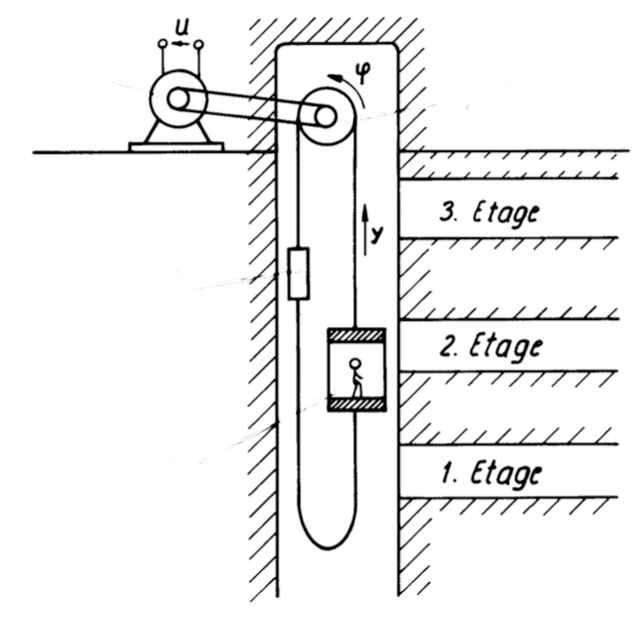
\includegraphics[width=3cm]{Aufzug.png}};
				%\fill (0,0) circle (2pt); % show origin
				% Destination coordinates
				\path (1.6, -0.5) coordinate (tscheibe)
						(0.6,-0.5) coordinate (motor)
						(1.2,-1.5) coordinate (ggewicht)
						(1.7,-2.1) coordinate (lift);
			\end{tikzpicture}
		\end{column}
	\end{columns}	

	% define overlays
	% Note the use of the overlay option. This is required when 
	% you want to access nodes in different pictures (in combination with remember picture).
	\begin{tikzpicture}[overlay]
		\path[->,RSTorange,thick] (item-tscheibe) edge [out=0, in=110] (tscheibe);
		\path[->,RSTgreen,thick] (item-motor) edge [out=0, in = 180] (motor);
		\path[->,RSTblue,thick] (item-ggewicht) edge [out=0, in = -170] (ggewicht);
		\path[->,RSTyellow,thick] (item-lift) edge [bend right] (lift);
	\end{tikzpicture}

\end{frame}

